\documentclass[ignorenonframetext]{beamer}
\usepackage[utf8]{inputenc}
\hypersetup{pdfpagemode=UseNone,pdfstartview=FitH}

\newenvironment{infobox}[1]
{\begin{beamerboxesrounded}[shadow=true]{#1}}
{\end{beamerboxesrounded}}

\usepackage{lmodern}
\usepackage[T1]{fontenc}
\usepackage[polish]{babel}
\usepackage[utf8]{inputenc}
\usepackage{graphicx}
\usepackage{listings}
\usepackage[normalem]{ulem}
\usepackage[babel=true]{microtype}

\usetheme{EastLansing}
\usecolortheme{spruce}

\setbeamertemplate{headline}{}
\setbeamertemplate{navigation symbols}{}

\title{Development Process as a Code}
\author{Marcin Drobik \& Maciej Nowak}
\date{6 listopada 2018}

\begin{document}

\begin{frame}
	\titlepage
	\centering
	
\includegraphics[width=3.5cm]{images/fp-space.png}
	
\includegraphics[width=3.5cm]{images/kp-labs.png}
	
\includegraphics[width=3.5cm]{images/pw-sat.png}
\end{frame}

\begin{frame}{O nas}
\begin{columns}

\column{0.5\textwidth}
\begin{itemize}
	\item "My" to:
	\begin{itemize}
		\item Marcin Drobik \texttt{SP9MNDR}
		\item Maciej Nowak \texttt{SP9NOV}
	\end{itemize}
	\item PW-Sat 2
	\begin{itemize}
		\item Czwarty Polski satelita
		\item \textbf{Start 19 listopada 2018!}
		\item Oprogramowanie komputera pokładowego
	\end{itemize} 
	\item Intuition-1
	\begin{itemize}
		\item Hiperspektralna obserwacja Ziemi
		\item Start Q4 2022
		\item Oprogramowanie komputera pokładowego i jednostki przetwarzającej
	\end{itemize} 
\end{itemize}

\column{0.5\textwidth}
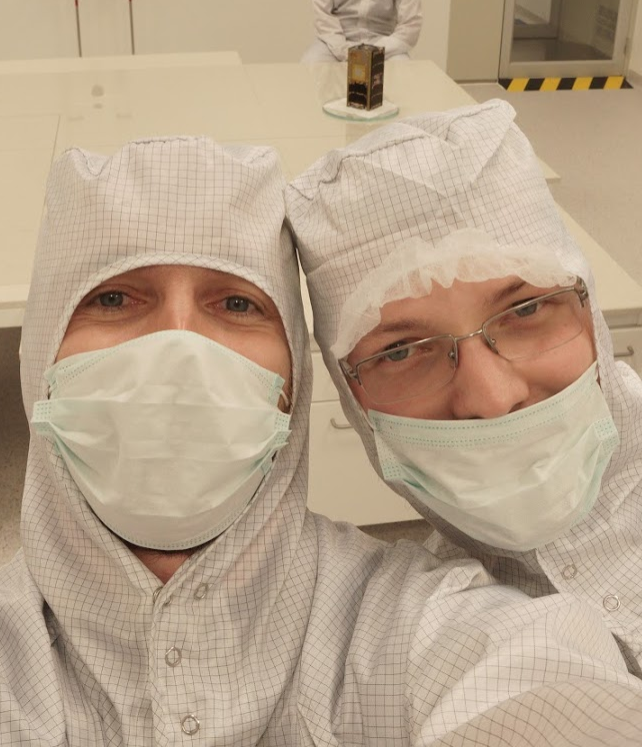
\includegraphics[scale=0.3]{images/we.png}
\end{columns}
\end{frame}

\begin{frame}{O czym jest ta prezentacja?}
\begin{itemize}
	\item Case Study: Używany przez nas proces i narzędzia
	\item Zarządzanie projektem: proces jako kod
	\item Dwa wątki: praktyka (wprowadzenie do projektu) i teoria (slajdy)
\end{itemize}
\end{frame}

\begin{frame}{DEMO}
\centering

\includegraphics[width=8cm]{images/first-contact.png}
\end{frame}

\begin{frame}{ŚBD - Ściągasz, Budujesz, Działasz}
\begin{itemize}
	\item Opis w \texttt{Readme}
	\item Szybki start dla nowych osób
	\item Podlega takiemu samemu procesowi jak kod
\end{itemize}
\end{frame}

\begin{frame}{DEMO}
	\centering
	
\includegraphics[width=8cm]{images/undiscovered-country.png}
\end{frame}

\begin{frame}{Git Flow}
\begin{itemize}
	\item Alternatywa: Feature Toggle
	\item Testy
	\begin{itemize}
		\item Rodzaje testów
		\item UI, Hardware - Da się! 
	\end{itemize}
	\item Testy kownencji
	\begin{itemize}
		\item Nazewnictwo
		\item Struktura
		\item Konfiguracja
	\end{itemize}
\end{itemize}
\end{frame}

\begin{frame}{DEMO}
	\centering
	
\includegraphics[width=8cm]{images/wrath-of-khan.png}
\end{frame}

\begin{frame}{Chat - Arek}
\begin{itemize}
	\item Bot 
	\item Przydziela ludzi do CR
	\item Pilnuje spójności między systemami (GitLab, JIRA)
	\item Odpalany z automatycznie lub na żądanie
\end{itemize}
\end{frame}

\begin{frame}{Continuous Integration}
\begin{itemize}
	\item Każdy branch
	\item Automatyczne wykrywanie niespójności (testy konwencji)
	\item Zepsuty build blokuje merge'a
	\item Izolacja testów
\end{itemize}
\end{frame}

\begin{frame}{Code Review - patologie}
\begin{columns}
	\begin{column}{0.45\textwidth}
		\begin{itemize}
			\item TL;DR: Looks good
			\item Nie znam CSS - wygląda ok
			\item Samoakceptacja rozwiązania
			\item Niekonstuktywna krytyka
		\end{itemize}
	\end{column}
	\begin{column}{0.55\textwidth}
		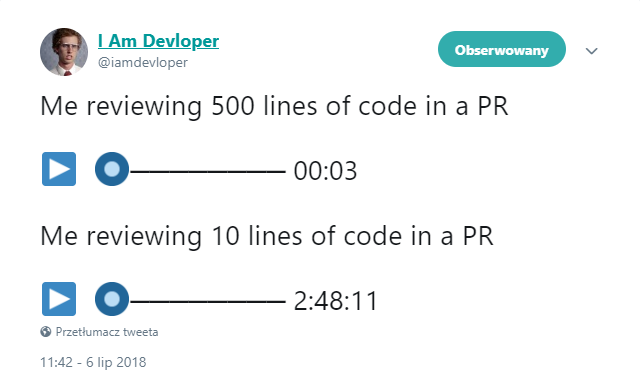
\includegraphics[width=7cm]{images/cr500lines.png}
	\end{column}
\end{columns}
\end{frame}

\begin{frame}{Code Review - ideał}
\begin{itemize}
	\item Komentarze są najważniejsze.
	\item Dobry diff:
	\begin{itemize} 
		\item Nie miesza zmian dokonanych w międzyczasie na docelowym branchu.
	\end{itemize}
	\item Przyrostowe review:
	\begin{itemize} 
		\item Następnym razem zobaczę tylko to co mnie interesuje.
	\end{itemize}
	\item Potwierdzanie przejrzenia każdego pliku osobno.
	\item Zaawansowana konfiguracja per project:
	\begin{itemize}
		\item ,,Potrzebne są akceptacje 2 osób''
		\item ,,Pliki w katalogu \texttt{Frontend} muszą być zaakceptowane przez \texttt{gbrzeczeszczykiewicz}''
	\end{itemize}
\end{itemize}
\end{frame}

\begin{frame}{Code Review - realia}

	\begin{columns}
	
	\begin{column}{0.3\textwidth}
		\centering
		
\includegraphics[scale=0.17]{images/chainsaw.png}
	\end{column}
	\begin{column}{0.7\textwidth}

		\LARGE
		CodeSaw
		\normalsize

		\begin{itemize}
			\item Brutalność
				\begin{itemize}
					\item Każdy plik przejrzany
					\item Każda dyskusja rozwiązana i potwierdzona
					\item Ścisły podział autor-reviewer
				\end{itemize}
			\item Odcięte niepotrzebne informacje (Inkrementacyjne review)
			\item Rozbudowana konfiguracja
			\item Integracja z Merge Requestami
		\end{itemize}
	\end{column}
\end{columns}
\end{frame}

\begin{frame}{Cośtamfile}
\begin{itemize}
	\item Dockerfile
	\item Makefile
	\item Jenkinsfile
	\item Arekfile
	\item Reviewfile
\end{itemize}
\end{frame}

\begin{frame}{DPasC - podsumowanie}
\begin{itemize}
	\item README jako punkt wejścia
	\item Ściągasz, Budujesz, Działasz	
	\item Opis procesu razem z kodem (śledzenie zmian)
	\item Testy na wszystko
	\item Kodyfikacja zasad (np. code review)
\end{itemize}
\end{frame}

\begin{frame}{DPasC - narzędzia}
Toolchain:
\begin{itemize}
	\item Rocket.Chat
	\item Hubot
	\item GitLab CE
	\item Jenkins
	\item JIRA
	\item \url{https://github.com/ChainsawDevelopment}
	\begin{itemize}
		\item Arek
		\item CodeSaw
	\end{itemize}
\end{itemize}

\end{frame}

\begin{frame}{Ewolucja procesu}
\begin{itemize}
	\item Proces jest jak kod - \sout{nie działa} zmienia się w czasie
	\item Zmiany w procesie muszą być jawne
	\item Zmiany w procesie powinny podlegać podobnym regułom co kod
		\begin{itemize}
			\item ...tak samo jak dokumentacja
			\item ...tak samo jak infrastruktura
		\end{itemize}
\end{itemize}
\end{frame}

\begin{frame}{To tyle}
\begin{center}
	
\includegraphics[scale=0.4]{images/thats-all.png}
	\tiny{https://commons.wikimedia.org/wiki/File:Thats\_all\_folks.svg}
\end{center}
\begin{beamerboxesrounded}{}
	\begin{center}
		\textbf{@mandrek44} SP9MNDR \textbf{@maciejt\_nowak} SP9NOV\\
		Przez: SR9EE SR9GC
	\end{center}
\end{beamerboxesrounded}
\end{frame}

\end{document}